% cd ~/storage/emulated/0/Documents/documents/latex/1920/Grade-8/2nd/functions/&& pdflatex hand-functions.tex && divide 1x2 hand-functions.pdf



\documentclass[handout]{beamer} 

\usepackage{pgfpages} 
\mode<handout>{%
\pgfpagesuselayout{4 on 1}[%letterpaper, 
legalpaper,% landscape, 
border shrink=1mm] 
}

\usepackage{xcolor}
\usepackage{anyfontsize}
\usepackage{enumitem}
\usepackage{multicol}
\usepackage{amsmath, makecell}
\usepackage{tabularx} 
\usepackage{gensymb}
\usepackage{wasysym} %for checked symbol 
\usepackage{multirow}
\usepackage{graphicx, tipa}
\usepackage{tikz}
\usetikzlibrary{angles,quotes}
\usepackage{pgfplots} 
\usetikzlibrary{calc}
\pgfplotsset{compat=newest}
\usetikzlibrary{arrows.meta}
\usetikzlibrary{intersections}
\usetikzlibrary{decorations.pathreplacing}
\usepackage{flafter}
%\usepackage{fourier} 
\usepackage{amsmath,amssymb,cancel,units}
\usepackage{microtype} % nicer output 
\usepackage{hfoldsty} % nicer output 
\usepackage{fixltx2e} 
\usepackage{mathptmx}
\usepackage{numprint}
\usepackage[T1]{fontenc}
\usepackage[utf8]{inputenc} 
\usepackage{stackengine} %to define \pesos 
\usepackage{lmodern} %scalable font
\usepackage{booktabs}
\usepackage{array}


\pagenumbering{gobble}
%\linespread{0.9}
\newcommand{\vspce}{\vspace{0.75ex}}

\newcommand{\hspce}{\hspace{0.5em}}

\newcommand{\blank}{\underline{\hspace{2em}}}%{\rule{1em}{0.15ex}}

\newcommand{\arc}[1]{{% 
\setbox9=\hbox{#1}% 
\ooalign{\resizebox{\wd9}{\height}{\texttoptiebar{\phantom{A}}}\cr#1}}}


\newcommand\pesos{\stackengine{-1.4ex}{P}{\stackengine{-1.25ex}{$-$}{$-$}{O}{c}{F}{F}{S}}{O}{c}{F}{T}{S}} 


\renewcommand\theadalign{bc} 

\renewcommand\theadfont{\bfseries} 

\renewcommand\theadgape{\Gape[4pt]} 

\renewcommand\cellgape{\Gape[4pt]} 

\pagenumbering{gobble}

\newcolumntype{Y}{>{\centering\arraybackslash}X} %for tabularx

\newcolumntype{R}{>{\raggedleft\arraybackslash}X} %for tabularx

\newcolumntype{Z}{>{\raggedleft\arraybackslash}X} %for tabularx

\newcolumntype{L}{>{\raggedright\arraybackslash}X} %for tabularx

\newcolumntype{A}[1]{>{\raggedright\arraybackslash}p{#1}} %for longtable LEFT

\newcolumntype{C}[1]{>{\centering\arraybackslash}p{#1}} %for longtable CENTER

\newcolumntype{B}[1]{>{\raggedleft\arraybackslash}p{#1}} %for longtable RIGHT 
 
\renewcommand{\tabularxcolumn}[1]{>{\small}m{#1}}

\newcolumntype{N}[1]{>{\raggedleft}p{#1}} %for tabular left 

\newcolumntype{M}[1]{>{\raggedright\arraybackslash}p{#1}} %for tabular right 

\newcommand{\myaxis}{xticklabels={}, 
yticklabels={}, 
ymin=-10, ymax=10,
xmin=-10, xmax=10,
axis lines = center, 
inner axis line style={Latex-Latex,very thick}, 
grid=both,
minor tick num=4, 
tick align=inside} % grid without labels, origin at the center, 10 units from origin

\newcommand{\axisfive}{xticklabels={}, 
yticklabels={}, 
ymin=-5, ymax=5,
xmin=-5, xmax=5,
axis lines = center, 
inner axis line style={Latex-Latex,very thick}, 
grid=both,
minor tick num=1, 
tick align=inside} % grid with labels, origin at the center, 5 units from origin 

\newcommand \redcheck {{\color{red}\checkmark}}



%\newcommand{\vertadjust}{\vspace*{-1.5in}} % for letterpaper
%\newcommand{\vertadjustb}{\vspace*{-1.5in}} % for letterpaper
\newcommand{\vertadjust}{\vspace*{-2.5in}} % for legalpaper
\newcommand{\vertadjustb}{\vspace*{-2.5in}} % for legalpaper

\def\gridscale{0.4}

\begin{document} 

% frame 1
\vertadjust
\begin{frame} 
\begin{center}
\textbf{Functions}
\end{center}

\vspace*{1ex}

Function: a relation in which each element of the domain is paired with exactly one element of the range
 
\vspce 

If the domain is being repeated, then the relation is not a function. 

\vspce 

Vertical line test: helps to determine whether a graph is a function or not
 \\
%\input{hand-functions-input1}
\textbf{Practice Exercises}
%\textbf{Problem Set}

\vspce

Determine the kind of relation and whether the relation is a function or a mere relation. 

A. Ordered Pairs 
 
\begin{enumerate}[label = \arabic*. ]
%\begin{multicols}{2}
%#1
\item \hspce  \{(2, 1), (5, 1), (3, 1), (1, 1)\}
%\vspce
%#2
\item \hspce  \{(0, 0), (1, -1), (-2, 2), (3, -3), (4, 4)\}

\item \hspce  \{(1, 1), (1, -1), (3, 0), (1, -4), (1, 4)\}

\item \hspce  \{(1, -2), (1, 3), (-2, 5), (-1, 2), (0, 6)\}

%\end{multicols}
\end{enumerate}
 
B. Table

\begin{enumerate}[label = \arabic*. ]
%\begin{multicols}{2}
%#1
\item \hspce  
\begin{tabular}{|c|c|c|c|c|c|}
%\begin{tabularx}{12em}{|X|X|X|X|X|X|}
\hline 
x & -5 & -3 & 0 & 3 & 5 \\
\hline 
y & -1 & -1 & -1 & -1 & -1 \\
\hline 
\end{tabular}

\item \hspce  
\begin{tabular}{|c|c|c|c|c|c|}
\hline 
x & -1 & -1 & -1 & -1 & -1 \\
\hline 
y & -10 & -5 & 0 & 5 & 10 \\
\hline 
\end{tabular}

\item \hspce  
\begin{tabular}{|c|c|c|c|c|c|}
\hline 
x & -2 & -1 & 0 & 1 & 2 \\
\hline 
y & 2 & 4 & 6 & 8 & 10 \\
\hline 
\end{tabular}

\item \hspce  
\begin{tabular}{|c|c|c|c|c|c|}
\hline 
x & -2 & -1 & 0 & 1 & 2 \\
\hline 
y & 0 & 1 & 3 & 0 & 3 \\
\hline 
\end{tabular}
 
\end{enumerate} 

%\item Graph

%\end{enumerate} 


\def \curdir {/host-rootfs/storage/emulated/0/Documents/documents/latex/1920/Grade-8/2nd/functions/f}

C. Graph

\begin{enumerate}[label = \arabic*. ]
\begin{multicols}{2}
%1
\item 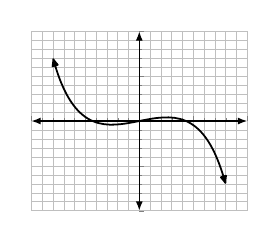
\begin{tikzpicture}[scale=\gridscale]

\begin{axis}[\myaxis] 

\draw[<->, >={Latex[round]},  ultra thick] (-8,7)..controls(-4,-9) and (4,9)..(8,-7);

\end{axis}
 
\end{tikzpicture}  
%2
\item 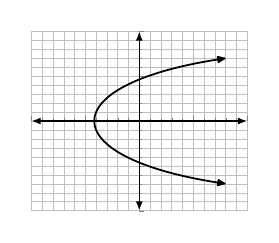
\begin{tikzpicture}[scale=\gridscale]

\begin{axis}[\myaxis] 

%\addplot[<->, >={Latex[round]},  ultra thick, domain=0:2.9, samples=200]{(x+1)^0.5}node[]{};

%\draw[color=blue] plot (\x,{sin(\x r)}); 
\draw[<->, >={Latex[round]},  ultra thick] (8,7)..controls(-8,4) and (-8,-4)..(8,-7);

\end{axis}
 
\end{tikzpicture} 
%3
\item 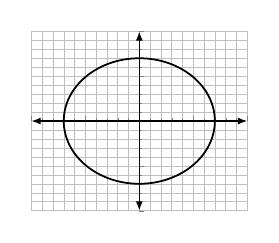
\begin{tikzpicture}[scale=\gridscale]

\begin{axis}[\myaxis] 

\draw[<->, >={Latex[round]},  ultra thick] (0,0) circle(7);

\end{axis}
 
\end{tikzpicture}  
%4
\item 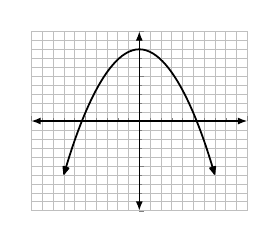
\begin{tikzpicture}[scale=\gridscale]

\begin{axis}[\myaxis] 

%\addplot[<->, >={Latex[round]},  ultra thick, domain=-1.6:2.6, samples=200]{x*(-x-1)*(x-1)*(x-2)}node[]{};
\draw[<->, >={Latex[round]},  ultra thick] (-7,-6) parabola bend (0,8) (7,-6);

\end{axis}
 
\end{tikzpicture} 
%5 
\item 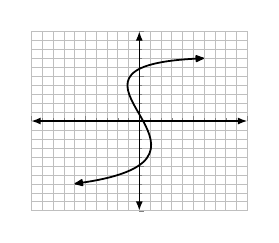
\begin{tikzpicture}[scale=\gridscale]

\begin{axis}[\myaxis] 

%\addplot[<->, >={Latex[round]},  ultra thick, domain=-3:1.8, samples=200]{(x+2)*(x+1)*(x-1)}node[]{};
\draw[<->, >={Latex[round]},  ultra thick] (6,7) .. controls (-11,6) and (11,-4) .. (-6,-7);
%\draw[<->, >={Latex[round]},  ultra thick] (6,7) .. controls (-6,6) and (-6,3) .. (4,3) ..  controls (6,-1) and (6,-4) ..(-6,-7);

\end{axis}
 
\end{tikzpicture}  
%6 
\item 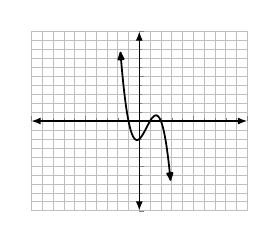
\begin{tikzpicture}[scale=\gridscale]

\begin{axis}[\myaxis] 

\addplot[<->, >={Latex[round]},  ultra thick, domain=-1.75:2.9, samples=200]{-(x+1)*(x-1)*(x-2)}node[]{};

\end{axis}
 
\end{tikzpicture} 
\end{multicols} 
\end{enumerate}  

%\def \curdir {/host-rootfs/storage/emulated/0/Documents/documents/latex/1920/Grade-8/2nd/functions/f}

%\textbf{Practice Exercises}
\textbf{Problem Set}

\vspce

Determine the kind of relation and whether the relation is a function or a mere relation. 

\begin{enumerate}[label = \Alph*. ]
\item Ordered Pairs 
 
\begin{enumerate}[label = \arabic*. ]
%\begin{multicols}{2}
%#1
\item \hspce  \{(3, 2), (4, 2), (5, 1), (6, 1)\}
%\vspce
%#2
\item \hspce  \{(0, 0), (-1, 1), (2, -2), (-3, 3)\}

\item \hspce  \{(2, 2), (2, -2), (4, 0), (2, -3), (2, 3)\}

\item \hspce  \{(2, -1), (1, 0), (0, 1), (-1, 2), (-2, 3)\}

\item \hspce  \{(2, 4), (1, 2), (0, 0), (-1, 2), (-2, 4)\}

%\end{multicols}
\end{enumerate}

\item Table

\begin{enumerate}[label = \arabic*. ]
%\begin{multicols}{2}
%#1
\item \hspce  
\begin{tabular}{|c|c|c|c|c|c|}
%\begin{tabularx}{12em}{|X|X|X|X|X|X|}
\hline 
x & -4 & -2 & 0 & 2 & 4 \\
\hline 
y & 1 & 1 & 1 & 1 & 1 \\
\hline 
\end{tabular}

\item \hspce  
\begin{tabular}{|c|c|c|c|c|c|}
\hline 
x & -2 & -1 & 0 & -1 & -2 \\
\hline 
y & -4 & -2 & 0 & 2 & 4 \\
\hline 
\end{tabular}

\item \hspce  
\begin{tabular}{|c|c|c|c|c|c|}
\hline 
x & -2 & -1 & 0 & 1 & 2 \\
\hline 
y & 3 & 4 & 5 & 6 & 7 \\
\hline 
\end{tabular}

\item \hspce  
\begin{tabular}{|c|c|c|c|c|c|}
\hline 
x & -3 & -1 & 0 & -1 & -3 \\
\hline 
y & 3 & 5 & 7 & 9 & 11 \\
\hline 
\end{tabular}

\item \hspce  
\begin{tabular}{|c|c|c|c|c|c|}
\hline 
x & -2 & -1 & 0 & 1 & 2 \\
\hline 
y & 0 & 1 & 2 & 3 & 4 \\
\hline 
\end{tabular}
 
\end{enumerate} 



\item Graph

\begin{enumerate}[label = \arabic*. ]
\begin{multicols}{2}
%1
\item 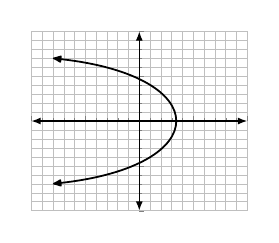
\begin{tikzpicture}[scale=\gridscale]

\begin{axis}[\myaxis] 

\draw[<->, >={Latex[round]},  ultra thick] (-8,-7)..controls(7,-5) and (7,5)..(-8,7);

\end{axis}
 
\end{tikzpicture} 
%2
\item 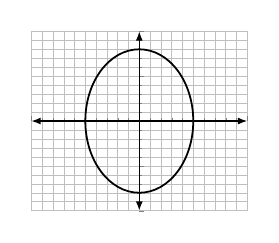
\begin{tikzpicture}[scale=\gridscale]

\begin{axis}[\myaxis] 

\draw[<->, >={Latex[round]},  ultra thick] (0,0) circle (5 and 8);

\end{axis}
 
\end{tikzpicture} 
%3
\item 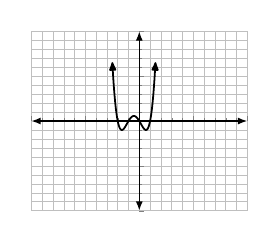
\begin{tikzpicture}[scale=\gridscale]

\begin{axis}[\myaxis] 

\addplot[<->, >={Latex[round]},  ultra thick, domain=-2.5:1.5, samples=200]{x*(x+2)*(x+1)*(x-1)}node[]{};

\end{axis}
 
\end{tikzpicture}  
%4
\item 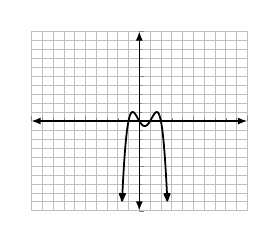
\begin{tikzpicture}[scale=\gridscale]

\begin{axis}[\myaxis] 

\addplot[<->, >={Latex[round]},  ultra thick, domain=-1.6:2.6, samples=200]{x*(-x-1)*(x-1)*(x-2)}node[]{};

\end{axis}
 
\end{tikzpicture} 
%5 
\item 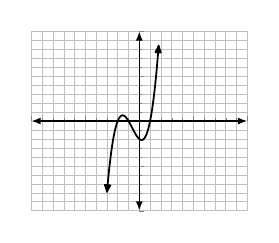
\begin{tikzpicture}[scale=\gridscale]

\begin{axis}[\myaxis] 

\addplot[<->, >={Latex[round]},  ultra thick, domain=-3:1.8, samples=200]{(x+2)*(x+1)*(x-1)}node[]{};

\end{axis}
 
\end{tikzpicture}  
%6 
\item 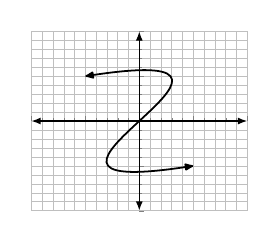
\begin{tikzpicture}[scale=\gridscale]

\begin{axis}[\myaxis] 

\draw[<->, >={Latex[round]},  ultra thick] (-5,5)..controls(17,9) and (-17,-9)..(5,-5);

\end{axis}
 
\end{tikzpicture} 
\end{multicols} 
\end{enumerate}  


\end{enumerate} 


\end{frame}

% frame 2
\vertadjust
\begin{frame} 
%\begin{center}
\textbf{Functions}
\end{center}

\vspace*{1ex}

Function: a relation in which each element of the domain is paired with exactly one element of the range
 
\vspce 

If the domain is being repeated, then the relation is not a function. 

\vspce 

Vertical line test: helps to determine whether a graph is a function or not
% \\
%\textbf{Practice Exercises}
%\textbf{Problem Set}

\vspce

Determine the kind of relation and whether the relation is a function or a mere relation. 

A. Ordered Pairs 
 
\begin{enumerate}[label = \arabic*. ]
%\begin{multicols}{2}
%#1
\item \hspce  \{(2, 1), (5, 1), (3, 1), (1, 1)\}
%\vspce
%#2
\item \hspce  \{(0, 0), (1, -1), (-2, 2), (3, -3), (4, 4)\}

\item \hspce  \{(1, 1), (1, -1), (3, 0), (1, -4), (1, 4)\}

\item \hspce  \{(1, -2), (1, 3), (-2, 5), (-1, 2), (0, 6)\}

%\end{multicols}
\end{enumerate}
 
B. Table

\begin{enumerate}[label = \arabic*. ]
%\begin{multicols}{2}
%#1
\item \hspce  
\begin{tabular}{|c|c|c|c|c|c|}
%\begin{tabularx}{12em}{|X|X|X|X|X|X|}
\hline 
x & -5 & -3 & 0 & 3 & 5 \\
\hline 
y & -1 & -1 & -1 & -1 & -1 \\
\hline 
\end{tabular}

\item \hspce  
\begin{tabular}{|c|c|c|c|c|c|}
\hline 
x & -1 & -1 & -1 & -1 & -1 \\
\hline 
y & -10 & -5 & 0 & 5 & 10 \\
\hline 
\end{tabular}

\item \hspce  
\begin{tabular}{|c|c|c|c|c|c|}
\hline 
x & -2 & -1 & 0 & 1 & 2 \\
\hline 
y & 2 & 4 & 6 & 8 & 10 \\
\hline 
\end{tabular}

\item \hspce  
\begin{tabular}{|c|c|c|c|c|c|}
\hline 
x & -2 & -1 & 0 & 1 & 2 \\
\hline 
y & 0 & 1 & 3 & 0 & 3 \\
\hline 
\end{tabular}
 
\end{enumerate} 

%\item Graph

%\end{enumerate} 


%\def \curdir {/host-rootfs/storage/emulated/0/Documents/documents/latex/1920/Grade-8/2nd/functions/f}

C. Graph

\begin{enumerate}[label = \arabic*. ]
\begin{multicols}{2}
%1
\item 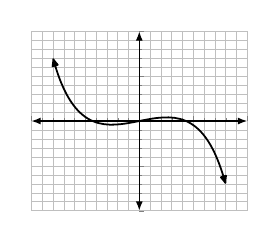
\begin{tikzpicture}[scale=\gridscale]

\begin{axis}[\myaxis] 

\draw[<->, >={Latex[round]},  ultra thick] (-8,7)..controls(-4,-9) and (4,9)..(8,-7);

\end{axis}
 
\end{tikzpicture}  
%2
\item 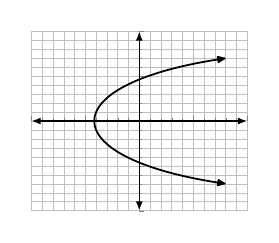
\begin{tikzpicture}[scale=\gridscale]

\begin{axis}[\myaxis] 

%\addplot[<->, >={Latex[round]},  ultra thick, domain=0:2.9, samples=200]{(x+1)^0.5}node[]{};

%\draw[color=blue] plot (\x,{sin(\x r)}); 
\draw[<->, >={Latex[round]},  ultra thick] (8,7)..controls(-8,4) and (-8,-4)..(8,-7);

\end{axis}
 
\end{tikzpicture} 
%3
\item 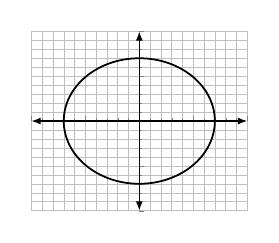
\begin{tikzpicture}[scale=\gridscale]

\begin{axis}[\myaxis] 

\draw[<->, >={Latex[round]},  ultra thick] (0,0) circle(7);

\end{axis}
 
\end{tikzpicture}  
%4
\item 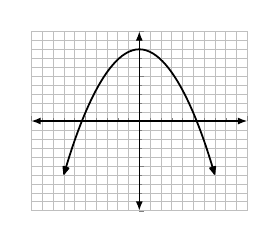
\begin{tikzpicture}[scale=\gridscale]

\begin{axis}[\myaxis] 

%\addplot[<->, >={Latex[round]},  ultra thick, domain=-1.6:2.6, samples=200]{x*(-x-1)*(x-1)*(x-2)}node[]{};
\draw[<->, >={Latex[round]},  ultra thick] (-7,-6) parabola bend (0,8) (7,-6);

\end{axis}
 
\end{tikzpicture} 
%5 
\item 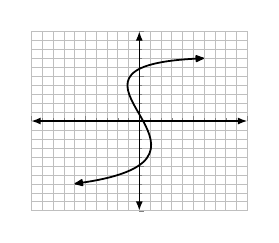
\begin{tikzpicture}[scale=\gridscale]

\begin{axis}[\myaxis] 

%\addplot[<->, >={Latex[round]},  ultra thick, domain=-3:1.8, samples=200]{(x+2)*(x+1)*(x-1)}node[]{};
\draw[<->, >={Latex[round]},  ultra thick] (6,7) .. controls (-11,6) and (11,-4) .. (-6,-7);
%\draw[<->, >={Latex[round]},  ultra thick] (6,7) .. controls (-6,6) and (-6,3) .. (4,3) ..  controls (6,-1) and (6,-4) ..(-6,-7);

\end{axis}
 
\end{tikzpicture}  
%6 
\item 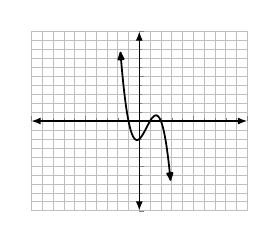
\begin{tikzpicture}[scale=\gridscale]

\begin{axis}[\myaxis] 

\addplot[<->, >={Latex[round]},  ultra thick, domain=-1.75:2.9, samples=200]{-(x+1)*(x-1)*(x-2)}node[]{};

\end{axis}
 
\end{tikzpicture} 
\end{multicols} 
\end{enumerate}  

%\input{hand-functions-input2}
\vspace*{1ex}
\def \curdir {/host-rootfs/storage/emulated/0/Documents/documents/latex/1920/Grade-8/2nd/functions/f}

%\textbf{Practice Exercises}
\textbf{Problem Set}

\vspce

Determine the kind of relation and whether the relation is a function or a mere relation. 

\begin{enumerate}[label = \Alph*. ]
\item Ordered Pairs 
 
\begin{enumerate}[label = \arabic*. ]
%\begin{multicols}{2}
%#1
\item \hspce  \{(3, 2), (4, 2), (5, 1), (6, 1)\}
%\vspce
%#2
\item \hspce  \{(0, 0), (-1, 1), (2, -2), (-3, 3)\}

\item \hspce  \{(2, 2), (2, -2), (4, 0), (2, -3), (2, 3)\}

\item \hspce  \{(2, -1), (1, 0), (0, 1), (-1, 2), (-2, 3)\}

\item \hspce  \{(2, 4), (1, 2), (0, 0), (-1, 2), (-2, 4)\}

%\end{multicols}
\end{enumerate}

\item Table

\begin{enumerate}[label = \arabic*. ]
%\begin{multicols}{2}
%#1
\item \hspce  
\begin{tabular}{|c|c|c|c|c|c|}
%\begin{tabularx}{12em}{|X|X|X|X|X|X|}
\hline 
x & -4 & -2 & 0 & 2 & 4 \\
\hline 
y & 1 & 1 & 1 & 1 & 1 \\
\hline 
\end{tabular}

\item \hspce  
\begin{tabular}{|c|c|c|c|c|c|}
\hline 
x & -2 & -1 & 0 & -1 & -2 \\
\hline 
y & -4 & -2 & 0 & 2 & 4 \\
\hline 
\end{tabular}

\item \hspce  
\begin{tabular}{|c|c|c|c|c|c|}
\hline 
x & -2 & -1 & 0 & 1 & 2 \\
\hline 
y & 3 & 4 & 5 & 6 & 7 \\
\hline 
\end{tabular}

\item \hspce  
\begin{tabular}{|c|c|c|c|c|c|}
\hline 
x & -3 & -1 & 0 & -1 & -3 \\
\hline 
y & 3 & 5 & 7 & 9 & 11 \\
\hline 
\end{tabular}

\item \hspce  
\begin{tabular}{|c|c|c|c|c|c|}
\hline 
x & -2 & -1 & 0 & 1 & 2 \\
\hline 
y & 0 & 1 & 2 & 3 & 4 \\
\hline 
\end{tabular}
 
\end{enumerate} 



\item Graph

\begin{enumerate}[label = \arabic*. ]
\begin{multicols}{2}
%1
\item 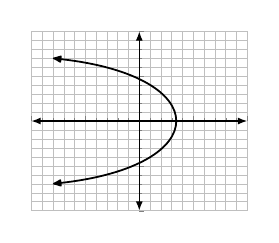
\begin{tikzpicture}[scale=\gridscale]

\begin{axis}[\myaxis] 

\draw[<->, >={Latex[round]},  ultra thick] (-8,-7)..controls(7,-5) and (7,5)..(-8,7);

\end{axis}
 
\end{tikzpicture} 
%2
\item 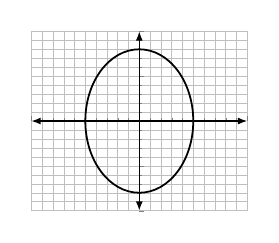
\begin{tikzpicture}[scale=\gridscale]

\begin{axis}[\myaxis] 

\draw[<->, >={Latex[round]},  ultra thick] (0,0) circle (5 and 8);

\end{axis}
 
\end{tikzpicture} 
%3
\item 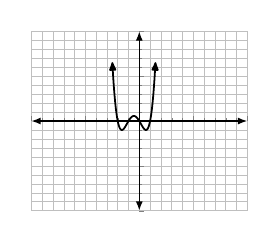
\begin{tikzpicture}[scale=\gridscale]

\begin{axis}[\myaxis] 

\addplot[<->, >={Latex[round]},  ultra thick, domain=-2.5:1.5, samples=200]{x*(x+2)*(x+1)*(x-1)}node[]{};

\end{axis}
 
\end{tikzpicture}  
%4
\item 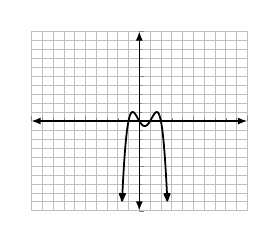
\begin{tikzpicture}[scale=\gridscale]

\begin{axis}[\myaxis] 

\addplot[<->, >={Latex[round]},  ultra thick, domain=-1.6:2.6, samples=200]{x*(-x-1)*(x-1)*(x-2)}node[]{};

\end{axis}
 
\end{tikzpicture} 
%5 
\item 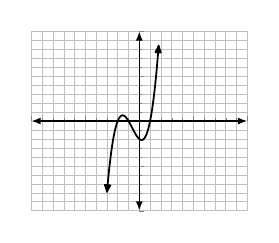
\begin{tikzpicture}[scale=\gridscale]

\begin{axis}[\myaxis] 

\addplot[<->, >={Latex[round]},  ultra thick, domain=-3:1.8, samples=200]{(x+2)*(x+1)*(x-1)}node[]{};

\end{axis}
 
\end{tikzpicture}  
%6 
\item 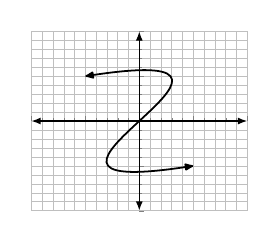
\begin{tikzpicture}[scale=\gridscale]

\begin{axis}[\myaxis] 

\draw[<->, >={Latex[round]},  ultra thick] (-5,5)..controls(17,9) and (-17,-9)..(5,-5);

\end{axis}
 
\end{tikzpicture} 
\end{multicols} 
\end{enumerate}  


\end{enumerate} 


\end{frame}

% frame 3
\vertadjustb
\begin{frame} 
\begin{center}
\textbf{Functions}
\end{center}

\vspace*{1ex}

Function: a relation in which each element of the domain is paired with exactly one element of the range
 
\vspce 

If the domain is being repeated, then the relation is not a function. 

\vspce 

Vertical line test: helps to determine whether a graph is a function or not
 \\
\textbf{Practice Exercises}
%\textbf{Problem Set}

\vspce

Determine the kind of relation and whether the relation is a function or a mere relation. 

A. Ordered Pairs 
 
\begin{enumerate}[label = \arabic*. ]
%\begin{multicols}{2}
%#1
\item \hspce  \{(2, 1), (5, 1), (3, 1), (1, 1)\}
%\vspce
%#2
\item \hspce  \{(0, 0), (1, -1), (-2, 2), (3, -3), (4, 4)\}

\item \hspce  \{(1, 1), (1, -1), (3, 0), (1, -4), (1, 4)\}

\item \hspce  \{(1, -2), (1, 3), (-2, 5), (-1, 2), (0, 6)\}

%\end{multicols}
\end{enumerate}
 
B. Table

\begin{enumerate}[label = \arabic*. ]
%\begin{multicols}{2}
%#1
\item \hspce  
\begin{tabular}{|c|c|c|c|c|c|}
%\begin{tabularx}{12em}{|X|X|X|X|X|X|}
\hline 
x & -5 & -3 & 0 & 3 & 5 \\
\hline 
y & -1 & -1 & -1 & -1 & -1 \\
\hline 
\end{tabular}

\item \hspce  
\begin{tabular}{|c|c|c|c|c|c|}
\hline 
x & -1 & -1 & -1 & -1 & -1 \\
\hline 
y & -10 & -5 & 0 & 5 & 10 \\
\hline 
\end{tabular}

\item \hspce  
\begin{tabular}{|c|c|c|c|c|c|}
\hline 
x & -2 & -1 & 0 & 1 & 2 \\
\hline 
y & 2 & 4 & 6 & 8 & 10 \\
\hline 
\end{tabular}

\item \hspce  
\begin{tabular}{|c|c|c|c|c|c|}
\hline 
x & -2 & -1 & 0 & 1 & 2 \\
\hline 
y & 0 & 1 & 3 & 0 & 3 \\
\hline 
\end{tabular}
 
\end{enumerate} 

%\item Graph

%\end{enumerate} 


\def \curdir {/host-rootfs/storage/emulated/0/Documents/documents/latex/1920/Grade-8/2nd/functions/f}

C. Graph

\begin{enumerate}[label = \arabic*. ]
\begin{multicols}{2}
%1
\item 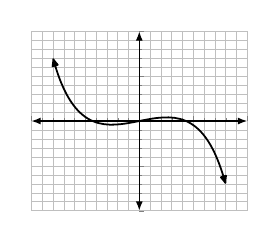
\begin{tikzpicture}[scale=\gridscale]

\begin{axis}[\myaxis] 

\draw[<->, >={Latex[round]},  ultra thick] (-8,7)..controls(-4,-9) and (4,9)..(8,-7);

\end{axis}
 
\end{tikzpicture}  
%2
\item 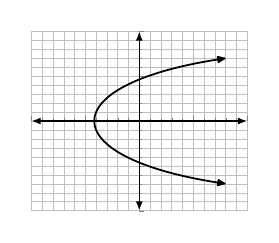
\begin{tikzpicture}[scale=\gridscale]

\begin{axis}[\myaxis] 

%\addplot[<->, >={Latex[round]},  ultra thick, domain=0:2.9, samples=200]{(x+1)^0.5}node[]{};

%\draw[color=blue] plot (\x,{sin(\x r)}); 
\draw[<->, >={Latex[round]},  ultra thick] (8,7)..controls(-8,4) and (-8,-4)..(8,-7);

\end{axis}
 
\end{tikzpicture} 
%3
\item 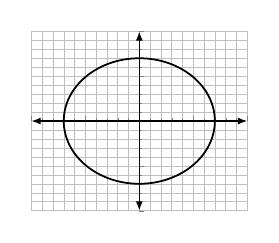
\begin{tikzpicture}[scale=\gridscale]

\begin{axis}[\myaxis] 

\draw[<->, >={Latex[round]},  ultra thick] (0,0) circle(7);

\end{axis}
 
\end{tikzpicture}  
%4
\item 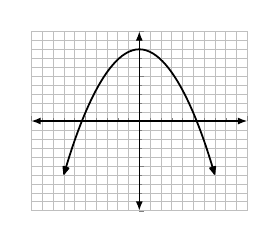
\begin{tikzpicture}[scale=\gridscale]

\begin{axis}[\myaxis] 

%\addplot[<->, >={Latex[round]},  ultra thick, domain=-1.6:2.6, samples=200]{x*(-x-1)*(x-1)*(x-2)}node[]{};
\draw[<->, >={Latex[round]},  ultra thick] (-7,-6) parabola bend (0,8) (7,-6);

\end{axis}
 
\end{tikzpicture} 
%5 
\item 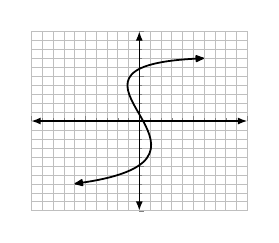
\begin{tikzpicture}[scale=\gridscale]

\begin{axis}[\myaxis] 

%\addplot[<->, >={Latex[round]},  ultra thick, domain=-3:1.8, samples=200]{(x+2)*(x+1)*(x-1)}node[]{};
\draw[<->, >={Latex[round]},  ultra thick] (6,7) .. controls (-11,6) and (11,-4) .. (-6,-7);
%\draw[<->, >={Latex[round]},  ultra thick] (6,7) .. controls (-6,6) and (-6,3) .. (4,3) ..  controls (6,-1) and (6,-4) ..(-6,-7);

\end{axis}
 
\end{tikzpicture}  
%6 
\item 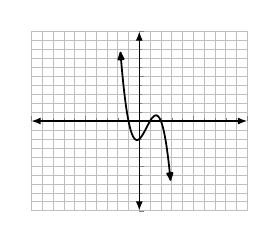
\begin{tikzpicture}[scale=\gridscale]

\begin{axis}[\myaxis] 

\addplot[<->, >={Latex[round]},  ultra thick, domain=-1.75:2.9, samples=200]{-(x+1)*(x-1)*(x-2)}node[]{};

\end{axis}
 
\end{tikzpicture} 
\end{multicols} 
\end{enumerate}  

%\def \curdir {/host-rootfs/storage/emulated/0/Documents/documents/latex/1920/Grade-8/2nd/functions/f}

%\textbf{Practice Exercises}
\textbf{Problem Set}

\vspce

Determine the kind of relation and whether the relation is a function or a mere relation. 

\begin{enumerate}[label = \Alph*. ]
\item Ordered Pairs 
 
\begin{enumerate}[label = \arabic*. ]
%\begin{multicols}{2}
%#1
\item \hspce  \{(3, 2), (4, 2), (5, 1), (6, 1)\}
%\vspce
%#2
\item \hspce  \{(0, 0), (-1, 1), (2, -2), (-3, 3)\}

\item \hspce  \{(2, 2), (2, -2), (4, 0), (2, -3), (2, 3)\}

\item \hspce  \{(2, -1), (1, 0), (0, 1), (-1, 2), (-2, 3)\}

\item \hspce  \{(2, 4), (1, 2), (0, 0), (-1, 2), (-2, 4)\}

%\end{multicols}
\end{enumerate}

\item Table

\begin{enumerate}[label = \arabic*. ]
%\begin{multicols}{2}
%#1
\item \hspce  
\begin{tabular}{|c|c|c|c|c|c|}
%\begin{tabularx}{12em}{|X|X|X|X|X|X|}
\hline 
x & -4 & -2 & 0 & 2 & 4 \\
\hline 
y & 1 & 1 & 1 & 1 & 1 \\
\hline 
\end{tabular}

\item \hspce  
\begin{tabular}{|c|c|c|c|c|c|}
\hline 
x & -2 & -1 & 0 & -1 & -2 \\
\hline 
y & -4 & -2 & 0 & 2 & 4 \\
\hline 
\end{tabular}

\item \hspce  
\begin{tabular}{|c|c|c|c|c|c|}
\hline 
x & -2 & -1 & 0 & 1 & 2 \\
\hline 
y & 3 & 4 & 5 & 6 & 7 \\
\hline 
\end{tabular}

\item \hspce  
\begin{tabular}{|c|c|c|c|c|c|}
\hline 
x & -3 & -1 & 0 & -1 & -3 \\
\hline 
y & 3 & 5 & 7 & 9 & 11 \\
\hline 
\end{tabular}

\item \hspce  
\begin{tabular}{|c|c|c|c|c|c|}
\hline 
x & -2 & -1 & 0 & 1 & 2 \\
\hline 
y & 0 & 1 & 2 & 3 & 4 \\
\hline 
\end{tabular}
 
\end{enumerate} 



\item Graph

\begin{enumerate}[label = \arabic*. ]
\begin{multicols}{2}
%1
\item 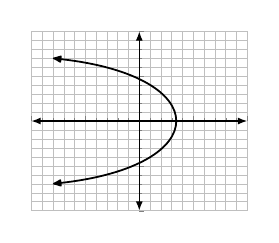
\begin{tikzpicture}[scale=\gridscale]

\begin{axis}[\myaxis] 

\draw[<->, >={Latex[round]},  ultra thick] (-8,-7)..controls(7,-5) and (7,5)..(-8,7);

\end{axis}
 
\end{tikzpicture} 
%2
\item 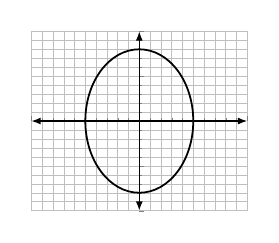
\begin{tikzpicture}[scale=\gridscale]

\begin{axis}[\myaxis] 

\draw[<->, >={Latex[round]},  ultra thick] (0,0) circle (5 and 8);

\end{axis}
 
\end{tikzpicture} 
%3
\item 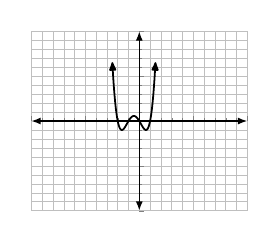
\begin{tikzpicture}[scale=\gridscale]

\begin{axis}[\myaxis] 

\addplot[<->, >={Latex[round]},  ultra thick, domain=-2.5:1.5, samples=200]{x*(x+2)*(x+1)*(x-1)}node[]{};

\end{axis}
 
\end{tikzpicture}  
%4
\item 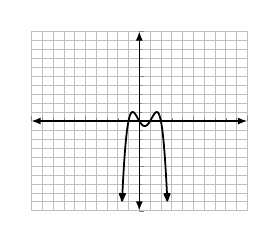
\begin{tikzpicture}[scale=\gridscale]

\begin{axis}[\myaxis] 

\addplot[<->, >={Latex[round]},  ultra thick, domain=-1.6:2.6, samples=200]{x*(-x-1)*(x-1)*(x-2)}node[]{};

\end{axis}
 
\end{tikzpicture} 
%5 
\item 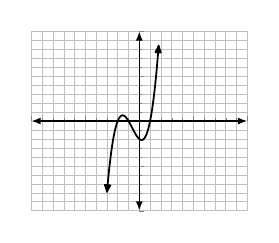
\begin{tikzpicture}[scale=\gridscale]

\begin{axis}[\myaxis] 

\addplot[<->, >={Latex[round]},  ultra thick, domain=-3:1.8, samples=200]{(x+2)*(x+1)*(x-1)}node[]{};

\end{axis}
 
\end{tikzpicture}  
%6 
\item 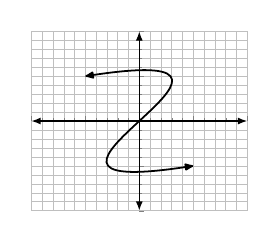
\begin{tikzpicture}[scale=\gridscale]

\begin{axis}[\myaxis] 

\draw[<->, >={Latex[round]},  ultra thick] (-5,5)..controls(17,9) and (-17,-9)..(5,-5);

\end{axis}
 
\end{tikzpicture} 
\end{multicols} 
\end{enumerate}  


\end{enumerate} 


\end{frame}

% frame 4
\vertadjustb
\begin{frame} 
%\begin{center}
\textbf{Functions}
\end{center}

\vspace*{1ex}

Function: a relation in which each element of the domain is paired with exactly one element of the range
 
\vspce 

If the domain is being repeated, then the relation is not a function. 

\vspce 

Vertical line test: helps to determine whether a graph is a function or not

%\textbf{Practice Exercises}
%\textbf{Problem Set}

\vspce

Determine the kind of relation and whether the relation is a function or a mere relation. 

A. Ordered Pairs 
 
\begin{enumerate}[label = \arabic*. ]
%\begin{multicols}{2}
%#1
\item \hspce  \{(2, 1), (5, 1), (3, 1), (1, 1)\}
%\vspce
%#2
\item \hspce  \{(0, 0), (1, -1), (-2, 2), (3, -3), (4, 4)\}

\item \hspce  \{(1, 1), (1, -1), (3, 0), (1, -4), (1, 4)\}

\item \hspce  \{(1, -2), (1, 3), (-2, 5), (-1, 2), (0, 6)\}

%\end{multicols}
\end{enumerate}
 
B. Table

\begin{enumerate}[label = \arabic*. ]
%\begin{multicols}{2}
%#1
\item \hspce  
\begin{tabular}{|c|c|c|c|c|c|}
%\begin{tabularx}{12em}{|X|X|X|X|X|X|}
\hline 
x & -5 & -3 & 0 & 3 & 5 \\
\hline 
y & -1 & -1 & -1 & -1 & -1 \\
\hline 
\end{tabular}

\item \hspce  
\begin{tabular}{|c|c|c|c|c|c|}
\hline 
x & -1 & -1 & -1 & -1 & -1 \\
\hline 
y & -10 & -5 & 0 & 5 & 10 \\
\hline 
\end{tabular}

\item \hspce  
\begin{tabular}{|c|c|c|c|c|c|}
\hline 
x & -2 & -1 & 0 & 1 & 2 \\
\hline 
y & 2 & 4 & 6 & 8 & 10 \\
\hline 
\end{tabular}

\item \hspce  
\begin{tabular}{|c|c|c|c|c|c|}
\hline 
x & -2 & -1 & 0 & 1 & 2 \\
\hline 
y & 0 & 1 & 3 & 0 & 3 \\
\hline 
\end{tabular}
 
\end{enumerate} 

%\item Graph

%\end{enumerate} 


%\def \curdir {/host-rootfs/storage/emulated/0/Documents/documents/latex/1920/Grade-8/2nd/functions/f}

C. Graph

\begin{enumerate}[label = \arabic*. ]
\begin{multicols}{2}
%1
\item 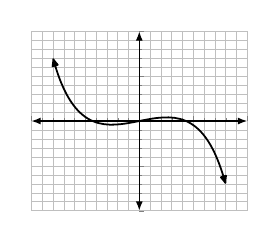
\begin{tikzpicture}[scale=\gridscale]

\begin{axis}[\myaxis] 

\draw[<->, >={Latex[round]},  ultra thick] (-8,7)..controls(-4,-9) and (4,9)..(8,-7);

\end{axis}
 
\end{tikzpicture}  
%2
\item 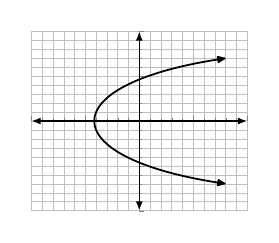
\begin{tikzpicture}[scale=\gridscale]

\begin{axis}[\myaxis] 

%\addplot[<->, >={Latex[round]},  ultra thick, domain=0:2.9, samples=200]{(x+1)^0.5}node[]{};

%\draw[color=blue] plot (\x,{sin(\x r)}); 
\draw[<->, >={Latex[round]},  ultra thick] (8,7)..controls(-8,4) and (-8,-4)..(8,-7);

\end{axis}
 
\end{tikzpicture} 
%3
\item 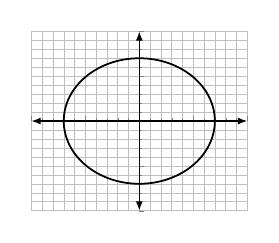
\begin{tikzpicture}[scale=\gridscale]

\begin{axis}[\myaxis] 

\draw[<->, >={Latex[round]},  ultra thick] (0,0) circle(7);

\end{axis}
 
\end{tikzpicture}  
%4
\item 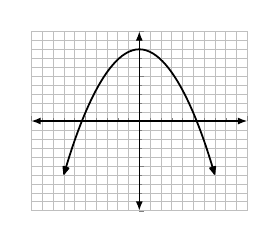
\begin{tikzpicture}[scale=\gridscale]

\begin{axis}[\myaxis] 

%\addplot[<->, >={Latex[round]},  ultra thick, domain=-1.6:2.6, samples=200]{x*(-x-1)*(x-1)*(x-2)}node[]{};
\draw[<->, >={Latex[round]},  ultra thick] (-7,-6) parabola bend (0,8) (7,-6);

\end{axis}
 
\end{tikzpicture} 
%5 
\item 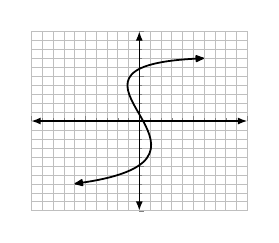
\begin{tikzpicture}[scale=\gridscale]

\begin{axis}[\myaxis] 

%\addplot[<->, >={Latex[round]},  ultra thick, domain=-3:1.8, samples=200]{(x+2)*(x+1)*(x-1)}node[]{};
\draw[<->, >={Latex[round]},  ultra thick] (6,7) .. controls (-11,6) and (11,-4) .. (-6,-7);
%\draw[<->, >={Latex[round]},  ultra thick] (6,7) .. controls (-6,6) and (-6,3) .. (4,3) ..  controls (6,-1) and (6,-4) ..(-6,-7);

\end{axis}
 
\end{tikzpicture}  
%6 
\item 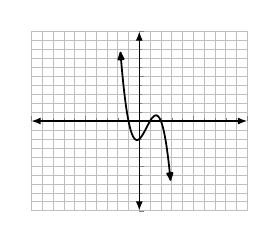
\begin{tikzpicture}[scale=\gridscale]

\begin{axis}[\myaxis] 

\addplot[<->, >={Latex[round]},  ultra thick, domain=-1.75:2.9, samples=200]{-(x+1)*(x-1)*(x-2)}node[]{};

\end{axis}
 
\end{tikzpicture} 
\end{multicols} 
\end{enumerate}  

%\input{hand-functions-input2}
\vspace*{1ex}
\def \curdir {/host-rootfs/storage/emulated/0/Documents/documents/latex/1920/Grade-8/2nd/functions/f}

%\textbf{Practice Exercises}
\textbf{Problem Set}

\vspce

Determine the kind of relation and whether the relation is a function or a mere relation. 

\begin{enumerate}[label = \Alph*. ]
\item Ordered Pairs 
 
\begin{enumerate}[label = \arabic*. ]
%\begin{multicols}{2}
%#1
\item \hspce  \{(3, 2), (4, 2), (5, 1), (6, 1)\}
%\vspce
%#2
\item \hspce  \{(0, 0), (-1, 1), (2, -2), (-3, 3)\}

\item \hspce  \{(2, 2), (2, -2), (4, 0), (2, -3), (2, 3)\}

\item \hspce  \{(2, -1), (1, 0), (0, 1), (-1, 2), (-2, 3)\}

\item \hspce  \{(2, 4), (1, 2), (0, 0), (-1, 2), (-2, 4)\}

%\end{multicols}
\end{enumerate}

\item Table

\begin{enumerate}[label = \arabic*. ]
%\begin{multicols}{2}
%#1
\item \hspce  
\begin{tabular}{|c|c|c|c|c|c|}
%\begin{tabularx}{12em}{|X|X|X|X|X|X|}
\hline 
x & -4 & -2 & 0 & 2 & 4 \\
\hline 
y & 1 & 1 & 1 & 1 & 1 \\
\hline 
\end{tabular}

\item \hspce  
\begin{tabular}{|c|c|c|c|c|c|}
\hline 
x & -2 & -1 & 0 & -1 & -2 \\
\hline 
y & -4 & -2 & 0 & 2 & 4 \\
\hline 
\end{tabular}

\item \hspce  
\begin{tabular}{|c|c|c|c|c|c|}
\hline 
x & -2 & -1 & 0 & 1 & 2 \\
\hline 
y & 3 & 4 & 5 & 6 & 7 \\
\hline 
\end{tabular}

\item \hspce  
\begin{tabular}{|c|c|c|c|c|c|}
\hline 
x & -3 & -1 & 0 & -1 & -3 \\
\hline 
y & 3 & 5 & 7 & 9 & 11 \\
\hline 
\end{tabular}

\item \hspce  
\begin{tabular}{|c|c|c|c|c|c|}
\hline 
x & -2 & -1 & 0 & 1 & 2 \\
\hline 
y & 0 & 1 & 2 & 3 & 4 \\
\hline 
\end{tabular}
 
\end{enumerate} 



\item Graph

\begin{enumerate}[label = \arabic*. ]
\begin{multicols}{2}
%1
\item 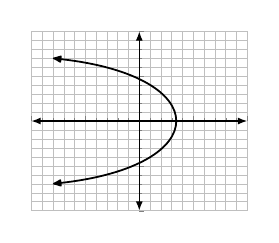
\begin{tikzpicture}[scale=\gridscale]

\begin{axis}[\myaxis] 

\draw[<->, >={Latex[round]},  ultra thick] (-8,-7)..controls(7,-5) and (7,5)..(-8,7);

\end{axis}
 
\end{tikzpicture} 
%2
\item 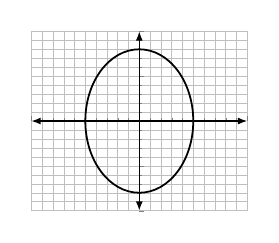
\begin{tikzpicture}[scale=\gridscale]

\begin{axis}[\myaxis] 

\draw[<->, >={Latex[round]},  ultra thick] (0,0) circle (5 and 8);

\end{axis}
 
\end{tikzpicture} 
%3
\item 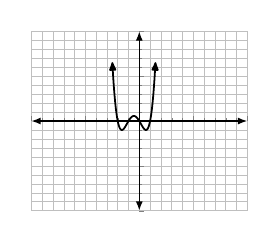
\begin{tikzpicture}[scale=\gridscale]

\begin{axis}[\myaxis] 

\addplot[<->, >={Latex[round]},  ultra thick, domain=-2.5:1.5, samples=200]{x*(x+2)*(x+1)*(x-1)}node[]{};

\end{axis}
 
\end{tikzpicture}  
%4
\item 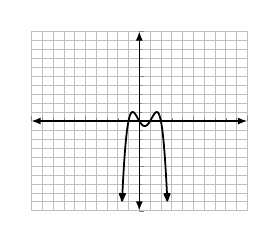
\begin{tikzpicture}[scale=\gridscale]

\begin{axis}[\myaxis] 

\addplot[<->, >={Latex[round]},  ultra thick, domain=-1.6:2.6, samples=200]{x*(-x-1)*(x-1)*(x-2)}node[]{};

\end{axis}
 
\end{tikzpicture} 
%5 
\item 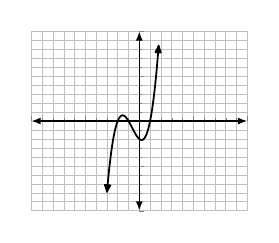
\begin{tikzpicture}[scale=\gridscale]

\begin{axis}[\myaxis] 

\addplot[<->, >={Latex[round]},  ultra thick, domain=-3:1.8, samples=200]{(x+2)*(x+1)*(x-1)}node[]{};

\end{axis}
 
\end{tikzpicture}  
%6 
\item 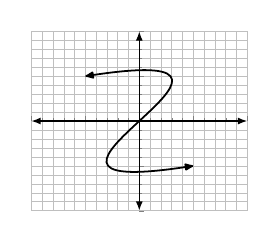
\begin{tikzpicture}[scale=\gridscale]

\begin{axis}[\myaxis] 

\draw[<->, >={Latex[round]},  ultra thick] (-5,5)..controls(17,9) and (-17,-9)..(5,-5);

\end{axis}
 
\end{tikzpicture} 
\end{multicols} 
\end{enumerate}  


\end{enumerate} 



\end{frame}

\end{document}

